% Slides adapted from notes_vNM/main.tex, in the style of introRL/main.tex.
%
% Reveals are \pause'd. Define \HANDOUT to collapse them into a static
% handout; the site build produces both variants (see docs/commands.md).
\ifdefined\HANDOUT\PassOptionsToClass{handout}{beamer}\fi
\documentclass[10pt,a4paper]{beamer}

\usepackage[utf8]{inputenc}
\usepackage[T1]{fontenc}
\usepackage{amsmath}
\usepackage{amsfonts}
\usepackage{amssymb}
\usepackage{mathtools}
\usepackage{graphicx}
\usetheme{Madrid}
\usepackage{xcolor}
\usepackage{tikz}
\usepackage{booktabs}
\usepackage{array}
\usepackage{hyperref}

\usetikzlibrary{arrows.meta, calc, positioning, shapes.geometric}

\hypersetup{
    colorlinks=true,
    linkcolor=white,
    filecolor=magenta,
    urlcolor=cyan,
}
\urlstyle{same}

\newcommand{\Hcal}{\mathcal{H}}
\newcommand{\Ofin}{\mathcal{O}}
\newcommand{\Afin}{\mathcal{A}}
\newcommand{\R}{\mathbb{R}}
\newcommand{\pref}{\succcurlyeq}
\newcommand{\strictpref}{\succ}
\newcommand{\indiff}{\sim}
\newcommand{\Lot}{\Delta}
\newcommand{\emptytraj}{\varepsilon}
\newcommand{\Ex}{\mathbb{E}}
\newcommand{\red}[1]{\textcolor{red}{#1}}
\newcommand{\blue}[1]{\textcolor{blue}{#1}}
\newcommand{\green}[1]{\textcolor{green!50!black}{#1}}
\newcommand{\transition}{T}
\newcommand{\exitem}{\item[$\triangleright$]}

\tikzset{
    box/.style={rectangle, rounded corners=2pt, draw=black!60, thick, align=center,
        minimum height=0.75cm, inner xsep=6pt, inner ysep=5pt},
    bigbox/.style={rectangle, rounded corners=3pt, draw=black!65, thick, align=center,
        minimum height=1.05cm, inner xsep=8pt, inner ysep=7pt},
    arrow/.style={-{Latex[length=2.2mm]}, thick},
    muted/.style={black!65},
    bluebox/.style={box, fill=blue!10, draw=blue!50!black},
    greenbox/.style={box, fill=green!10, draw=green!45!black},
    redbox/.style={box, fill=red!10, draw=red!55!black},
    goldbox/.style={box, fill=yellow!16, draw=orange!70!black},
}

\title[From preferences to rewards]
{From preferences to rewards: A brief introduction}

\author[F. Rosas]
{Fernando E. Rosas}

\institute[Iliad]
{
  Iliad Intensive
}

%\date[\today]{\today}

\begin{document}

\frame{\titlepage}

\begin{frame}
\frametitle{The Question}
\begin{itemize}
    \item Agents are powerful --- but increasing capabilities lead to increasing risks.
    \pause
    \item To understand agentic risk, we need to understand how agents work.
    \pause
    \item Core of agency: \textit{doing things (planning) for reasons (beliefs)}.
    \pause
    \item What are goals? Hard question.
    \pause
    \item \textbf{Goal of today}: understand what are preferences.
\end{itemize}
\end{frame}

\begin{frame}
\frametitle{The Route}
\centering
\resizebox{\linewidth}{!}{%
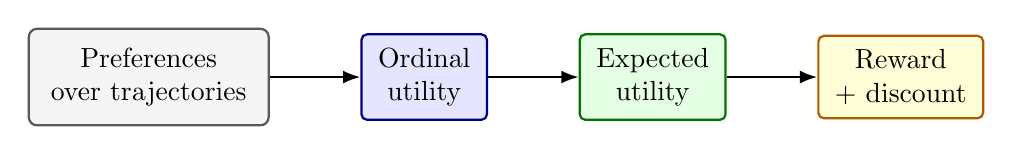
\begin{tikzpicture}[node distance=1.15cm]
    \node[bigbox, fill=gray!8] (pref) {Preferences\\over trajectories};
    \node[bigbox, bluebox, right=of pref] (ord) {Ordinal\\utility};
    \node[bigbox, greenbox, right=of ord] (vnm) {Expected\\utility};
    \node[bigbox, goldbox, right=of vnm] (reward) {Reward\\+ discount};
    \draw[arrow] (pref) -- (ord);
    \draw[arrow] (ord) -- (vnm);
    \draw[arrow] (vnm) -- (reward);
\end{tikzpicture}
}

\vspace{0.65cm}
\begin{itemize}
    \item Each arrow adds structure.
    \pause
    \item Each structure buys a more specific representation.
    \pause
    \item \textit{Outcome 1}: Understand the assumptions of each step.
    \pause
    \item \textit{Outcome 2}: Recognise the difference between preference, utility, and reward.
\end{itemize}
\end{frame}

\begin{frame}
\frametitle{Basic setting}
\begin{itemize}
    \item Let $\Ofin$ be a finite observation set, and $\Afin$ a finite action set.
    \pause
    \item A one-step interaction is
    $$
    t=(o,a)\in \Ofin\times \Afin.
    $$
    \pause
    \item A finite trajectory of length $n$ is
    $$
    h=(o_1,a_1,o_2,a_2,\dots,o_n,a_n)\in(\Ofin\times\Afin)^n.
    $$
    \pause
    \item The full finite trajectory space is
    $$
    \Hcal^*=\bigcup_{n=0}^{\infty}(\Ofin\times\Afin)^n.
    $$
\end{itemize}
\end{frame}

\begin{frame}
\frametitle{Preferences}
\begin{itemize}
    \item A weak preference relation $\pref$ compares complete trajectories.
    $$
    h\pref h'
    $$
    means ``$h$ is at least as good as $h'$.''
    \pause
    \item From this we define:
    \begin{align*}
        h \indiff h' &\iff h\pref h'\text{ and }h'\pref h,\\
        h \strictpref h' &\iff h\pref h'\text{ and not }h'\pref h.
    \end{align*}
    \pause
    \item At this point, $\pref$ need not be complete, transitive, numerical,
    or `reward-like'.
\end{itemize}
\end{frame}


\begin{frame}
\frametitle{Three Kinds of Trouble}
By choosing the ``wrong type of preference'', an agent can run into three kinds of trouble (from less to more harmful):
\vspace{0.4cm}
\begin{itemize}
    \item \textbf{Representability failure:}
    preference has no convenient formal representation.
    \pause
    \item \textbf{Self-defeat:}
    agents take suboptimal choices or plans --- there are better alternatives that are not being taken.
    \pause
    \begin{itemize}
        \exitem E.g.\ \textbf{dominance}: another policy yields preferred trajectories at least as preferred in every state of the world, and strictly so in at least one.
    \end{itemize}
    \pause
    \item \textbf{Vulnerability:}
    individually acceptable trades can combine into guaranteed loss.
    \begin{itemize}
        \exitem E.g.\ \textbf{Money pumps}: circular preferences ($h_1\strictpref h_2\strictpref h_3\strictpref h_1$) lead to indefinite loss.
    \end{itemize}
\end{itemize}
\end{frame}


\begin{frame}
    \frametitle{Money Pump Picture}
    \centering
    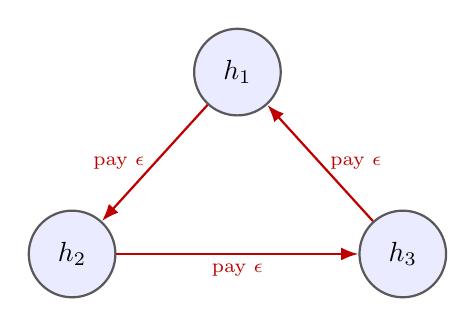
\begin{tikzpicture}[scale=1.05]
        \node[circle, draw=black!65, thick, fill=blue!8, minimum size=1.1cm] (h1) at (0,2.2) {$h_1$};
        \node[circle, draw=black!65, thick, fill=blue!8, minimum size=1.1cm] (h2) at (-2,0) {$h_2$};
        \node[circle, draw=black!65, thick, fill=blue!8, minimum size=1.1cm] (h3) at (2,0) {$h_3$};
        \draw[arrow, red!75!black] (h1) -- node[left, font=\scriptsize] {pay $\epsilon$} (h2);
        \draw[arrow, red!75!black] (h2) -- node[below, font=\scriptsize] {pay $\epsilon$} (h3);
        \draw[arrow, red!75!black] (h3) -- node[right, font=\scriptsize] {pay $\epsilon$} (h1);
    \end{tikzpicture}
    
    \vspace{0.35cm}
    \begin{itemize}
        \item If the agent pays for every strict improvement, a cycle can be exploited.
        \pause
        \item It returns to the same trajectory with less money.
        \pause
        \item Parallel with thermodynamics: the second law of thermodynamics can be read as stating that \textit{`nature cannot be money-pumped'}.
    \end{itemize}
    \end{frame}
    
    

\begin{frame}
\frametitle{Three Kinds of Results}
There are three types of results regarding preferences:
\vspace{0.4cm}
\begin{itemize}
    \item \textbf{Representation results:}
    axioms imply that preferences can be written in a particular mathematical form.
    \begin{itemize}
        \exitem E.g.\ some preferences can be represented as if maximising a utility function.
    \end{itemize}
    \pause
    \item \textbf{Coherence results:}
    violations imply some penalty for the agent.
    \begin{itemize}
        \exitem E.g.\ money pumps or Dutch books.
    \end{itemize}
    \pause
    \item \textbf{Selection results:}
    some optimization pressure tends to remove agents with a given failure mode.
    \begin{itemize}
        \exitem E.g.\ market competition or natural evolution.
    \end{itemize}
    \pause
\end{itemize}
These results are related (one can lead to the other) but not identical: form, vulnerability, and survival
    are different claims.
\end{frame}




\begin{frame}
\frametitle{Axiom 1: Completeness}
Completeness says every pair can be compared:
    $$
    \forall h,h'\in\Hcal^*,\qquad h\pref h'
    \quad\text{or}\quad h'\pref h.
    $$
\pause
\begin{itemize}
    \item Incomparability is not the same as indifference.
    \pause
    \item If it fails, some trajectories are genuinely incomparable.
\end{itemize}
\end{frame}

\begin{frame}
\frametitle{Axiom 2: Transitivity}
Transitivity says comparisons fit together:
    $$
    h\pref h'\text{ and }h'\pref h''
    \quad\Longrightarrow\quad
    h\pref h''.
    $$
    \pause
\begin{itemize}
    \item If it fails, local pairwise judgments need not form a global ranking.
    \pause
    \item The classic failure is a cycle: money pumps.
    $$
    h_1\strictpref h_2,\qquad
    h_2\strictpref h_3,\qquad
    h_3\strictpref h_1.
    $$
    \item Similar to Helmholtz-Hodge decomposition: transitivity is equivalent to requiring no rotational component.
\end{itemize}
\end{frame}



\begin{frame}
\frametitle{Axioms 1 + 2 $\to$ Ordinal Utility}
\begin{itemize}
    \item Completeness + transitivity make $\pref$ a weak order (total order with equivalent objects).
    \pause
    \item On a countable space $\Hcal^*$, weak orders admit an ordinal utility: 
    there exists a function $u:\Hcal^*\to\R$ such that
    $$
    h\pref h'
    \quad\Longleftrightarrow\quad
    u(h)\geq u(h').
    $$
    \pause
    \item Only the ranking matters:
    $$
    u,\quad 2u+17,\quad \exp(u)
    $$
    all represent the same deterministic preferences.
\end{itemize}
\end{frame}



\begin{frame}
\frametitle{Beyond Ordinal Utility}
Ordinal utility ranks outcomes, but gives a structure to mixtures of them.
\vspace{0.4cm}
\begin{itemize}
    \item Example:
    $$
    x\strictpref y\strictpref z.
    $$
    How should we rank $y$ with respect to
    $\tfrac12 x+\tfrac12 z$? Should they be equivalent?
    \pause
\end{itemize}
\vspace{0.4cm}
Ordinal rank doesn't say how to rank mixtures, which can arise naturally out of uncertainty.
\end{frame}

\begin{frame}
\frametitle{Lotteries Over Trajectories}
\begin{itemize}
    \item Let $\Lot(X)$ be the set of probability distributions over
    $X\subseteq \Hcal^*$.
    \pause
    \item A lottery is written
    $$
    \mu=\sum_i p_i\delta_{x_i}.
    $$
    \pause
    \item A sure trajectory $x$ is the degenerate lottery $\delta_x$.
    \pause
    \item We can mix lotteries:
    $$
    \lambda\mu+(1-\lambda)\nu.
    $$
\end{itemize}
\end{frame}

\begin{frame}
\frametitle{Lottery Picture}
\centering
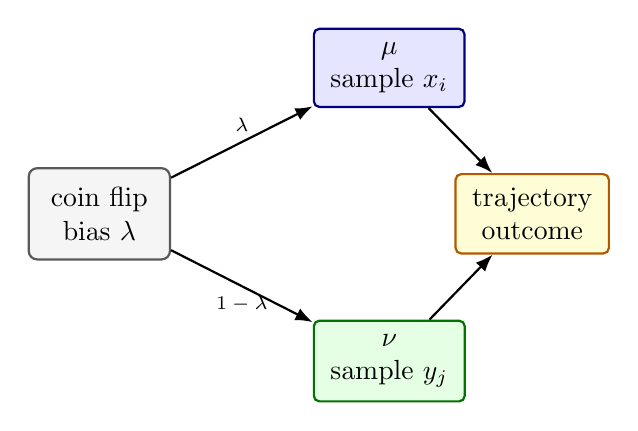
\begin{tikzpicture}[node distance=1.25cm]
    \node[bigbox, fill=gray!8] (coin) {coin flip\\bias $\lambda$};
    \node[bigbox, bluebox, above right=0.75cm and 1.8cm of coin] (mu) {$\mu$\\sample $x_i$};
    \node[bigbox, greenbox, below right=0.75cm and 1.8cm of coin] (nu) {$\nu$\\sample $y_j$};
    \node[bigbox, goldbox, right=3.6cm of coin] (out) {trajectory\\outcome};
    \draw[arrow] (coin) -- node[above, font=\scriptsize] {$\lambda$} (mu);
    \draw[arrow] (coin) -- node[below, font=\scriptsize] {$1-\lambda$} (nu);
    \draw[arrow] (mu) -- (out);
    \draw[arrow] (nu) -- (out);
\end{tikzpicture}

\vspace{0.55cm}
\begin{itemize}
    \item vNM asks when preferences over these objects are expectations.
\end{itemize}
\end{frame}

\begin{frame}
\frametitle{vNM representation: The big picture}
\begin{enumerate}
    \item \textbf{Axiom 1: Completeness:} any two lotteries can be compared.
    \pause
    \item \textbf{Axiom 2: Transitivity:} comparisons over lotteries fit together.
    \pause
    \item \textbf{Axiom 3: Continuity:} intermediate prospects can be matched by a
    mixture of better and worse prospects.
    \pause
    \item \textbf{Axiom 4: Independence:} common lottery components cancel.
\end{enumerate}

\pause
\vspace{0.25cm}
\textbf{Result:}
The first two axioms give ranking structure based on an ordinal utility;
the last two axioms make the utility an expected value.
\end{frame}

\begin{frame}
\frametitle{Axiom 3: Continuity}
\begin{itemize}
    \item If $\mu\pref\nu\pref\xi$, 
    continuity says there always exists some value $\lambda\in[0,1]$ such that
    $$
    \nu\indiff \lambda\mu+(1-\lambda)\xi.
    $$
    \pause
    \item Intuition: no outcome is infinitely better or worse than the others.
    \pause
\end{itemize}
\vspace{0.4cm}
Classic counter-examples are lexicographic preferences, in which even the slimmest
chance of a catastrophically bad outcome is worse than a slightly bad outcome
with certianty, no matter how low the odds are.
\vspace{0.4cm}

\textit{Example}: $\mu$ is eating chocolate, $\nu$ is eating potatoes, and $\xi$ is accepting genocide.
\end{frame}



\begin{frame}
\frametitle{Axiom 4: Independence}
\begin{itemize}
    \item If $\mu\pref\nu$, then mixing both with the same background lottery
    $\xi$ should not reverse the comparison:
    $$
    \mu\pref\nu
    \Longleftrightarrow
    \lambda\mu+(1-\lambda)\xi
    \pref
    \lambda\nu+(1-\lambda)\xi.
    $$
    \pause
    \item Independence is what gives linear averaging.
    \pause
\end{itemize}
When it fails, common consequences do not psychologically or behaviorally cancel.
\vspace{0.4cm}

\textit{Example (Allais paradox):} Most people would say
\begin{itemize}
    \item Getting \$100 for sure \textit{is better than} a coin flip for \$250.
    \item A 1-in-100 shot at \$100 \textit{is worse than} a 1-in-200 shot at \$250.
\end{itemize}
These are the same choice, just scaled down.
\end{frame}


\begin{frame}
\frametitle{Theorem 1: The von Neumann--Morgenstern representation}

Assumptions: a finite set of options $X\subseteq\Hcal^*$, 
the four axioms hold.
\begin{itemize}
    \item  \textbf{Result 1 (existence):} there exists $u:X\to\R$ such that
    $$
    \mu\pref\nu
    \Longleftrightarrow
    \sum_{x\in X}\mu(x)u(x)
    \geq
    \sum_{x\in X}\nu(x)u(x).
    $$
    \pause
    \item \textbf{Result 2 (uniqueness):} $u$ is unique up to positive affine transformations:
    $$
    u'(x)=a+bu(x),\qquad b>0.
    $$
\end{itemize}
\end{frame}

\begin{frame}
\frametitle{Ordinal vs expected utility}
\begin{columns}
\begin{column}{0.48\textwidth}
\textbf{Ordinal utility}
\begin{itemize}
    \item Any set of outcomes
    \item Preserves ranking
    \item Indiferent to non-decreasing transformation
    \item Cannot display `meaningful gaps'
\end{itemize}
\end{column}
\begin{column}{0.48\textwidth}
\textbf{vNM utility}
\begin{itemize}
    \item Lotteries (probabilistic mixtures)
    \item Preserves risky choices
    \item Only affine transforms are okay
    \item Incommensurable gaps can exist
\end{itemize}
\end{column}
\end{columns}

\pause
\vspace{0.4cm}
\centering
vNM utility further refines ordinal utility (it is not just a relabeling).
\end{frame}



\begin{frame}
\frametitle{Beyond expected utility: Temporal structure}
\begin{itemize}
    \item vNM utility assigns a single scalar to a whole trajectory.
    \pause
    \item But agents make decisions over time, so they need indications of utility that unfold step-by-step.
    \pause
    \item From a global utility $u(h)$, one can always define the increment
    $$
    r(t;h)=u(t\cdot h)-u(h),\quad\text{satisfying}\quad u(t\cdot h)=r(t;h)+u(h).
    $$
    \begin{center}
    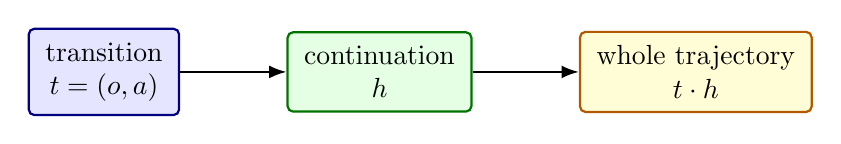
\begin{tikzpicture}[node distance=1.35cm]
    \node[bigbox, bluebox] (t) {transition\\$t=(o,a)$};
    \node[bigbox, greenbox, right=of t] (h) {continuation\\$h$};
    \node[bigbox, goldbox, right=of h] (th) {whole trajectory\\$t\cdot h$};
    \draw[arrow] (t) -- (h);
    \draw[arrow] (h) -- (th);
    \end{tikzpicture}
    \end{center}
    \pause
    \item But the increment $r(t;h)$ may be non-local, and hence cannot be optimised for directly.
\end{itemize}
\end{frame}


\begin{frame}
\frametitle{Axiom 5: Temporal equanimity}
Let $T=\Ofin\times\Afin$ be the transition set.
\begin{itemize}
    \item The fifth axiom says there is a function $\gamma:T\to[0,1]$ such that
    prepending $t$ rescales continuation differences, so that
    $$
    u(t\cdot\mu)-u(t\cdot\nu)
    =
    \gamma(t)\bigl(u(\mu)-u(\nu)\bigr).
    $$
\end{itemize}
$\gamma(t)$ measures how much the future still matters after $t$. 
\vspace{0.1cm}
\pause
\begin{itemize}
    \item $\gamma(t)=1$: future differences matter as much as present differences.
    \pause
    \item $0<\gamma(t)<1$: future differences are damped.
    \pause
    \item $\gamma(t)=0$: after $t$, continuation does not matter.
\end{itemize}
This is transition-dependent discounting, not necessarily a single
global constant.
\end{frame}


\begin{frame}
\frametitle{Theorem 2: Markov reward representation}
Assumptions: Axioms 1-5 over lotteries over trajectories.
\begin{itemize}
    \item Then, utility has a local recursive form:
    $$
    u(t\cdot h)=r(t)+\gamma(t)u(h),
    \qquad
    u(\emptytraj)=0.
    $$
    \pause
    \item Preferences over lotteries are still represented by expected utility.
    \pause
\end{itemize}
This establishes a bridge from expected utility maximisation over whole-trajectory utility 
to RL-style expected sum of future reward maximisation.
\end{frame}

\begin{frame}
\frametitle{Unrolling the recursion}
\begin{itemize}
    \item For $h=(t_1,t_2,\dots,t_n)$:
    \begin{align*}
    u(h)
    &= r(t_1)+\gamma(t_1)r(t_2)\\
    &\quad+\gamma(t_1)\gamma(t_2)r(t_3)+\cdots\\
    &\quad+\left(\prod_{i=1}^{n-1}\gamma(t_i)\right)r(t_n).
    \end{align*}
    \pause
    \item If $\gamma(t)\equiv\gamma$, this becomes standard discounted return:
    $$
    u(h)=\sum_{k=1}^n\gamma^{k-1}r(t_k).
    $$
\end{itemize}
\end{frame}

\begin{frame}
\frametitle{Summary: Preference, utility, and reward}
\centering
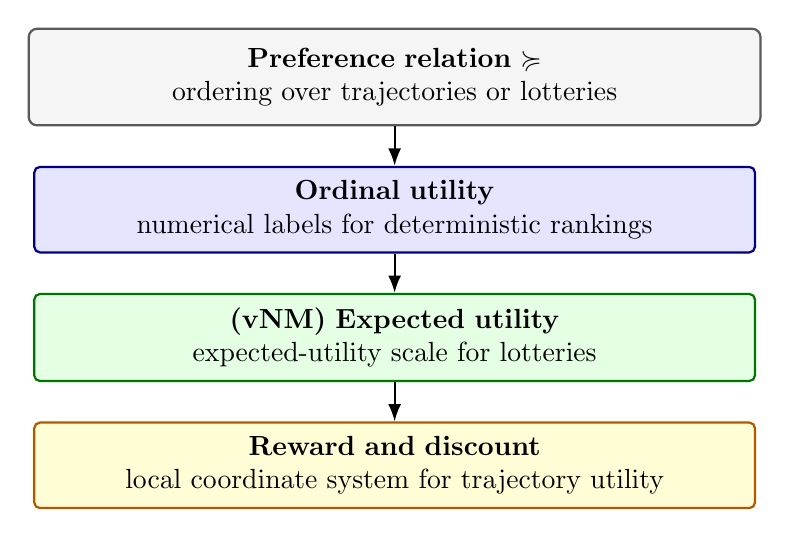
\begin{tikzpicture}[node distance=0.5cm]
    \node[bigbox, fill=gray!8, text width=0.72\linewidth] (pref) {
        \textbf{Preference relation} $\pref$\\
        ordering over trajectories or lotteries
    };
    \node[bigbox, bluebox, text width=0.72\linewidth, below=of pref] (uord) {
        \textbf{Ordinal utility}\\
        numerical labels for deterministic rankings
    };
    \node[bigbox, greenbox, text width=0.72\linewidth, below=of uord] (uvnm) {
        \textbf{(vNM) Expected utility}\\
        expected-utility scale for lotteries
    };
    \node[bigbox, goldbox, text width=0.72\linewidth, below=of uvnm] (reward) {
        \textbf{Reward and discount}\\
        local coordinate system for trajectory utility
    };
    \draw[arrow] (pref) -- (uord);
    \draw[arrow] (uord) -- (uvnm);
    \draw[arrow] (uvnm) -- (reward);
\end{tikzpicture}
\end{frame}


\begin{frame}
\frametitle{Open questions regarding AI alignment}
\begin{itemize}
    \item Will powerful AIs necessarily become expected utility maximisers?
    \pause
    \item Instead of `given a reward, how to optimise it' we could ask `what kind of properties we want our reward to satisfy'. For example, are any of these properties (or their negation) useful for fostering:
    \begin{itemize}
        \item Corrigibility? (e.g. incompleteness)
        \pause
        \item Robust values? (e.g. continuity)
        \pause
        \item Something else?
    \end{itemize}
    \item Is RLHF providing an ordinal or cardinal utility signal? Are there implications of this?
    \pause
\end{itemize}
\end{frame}



%
%\begin{frame}
%\frametitle{Reward Is Not Unique}
%\begin{itemize}
%    \item If $u$ and $\gamma$ are fixed, then
%    $$
%    r(t)=u(t\cdot h)-\gamma(t)u(h)
%    $$
%    is fixed and independent of $h$.
%    \pause
%    \item But vNM utility itself is only defined up to affine transformation.
%    \pause
%    \item If
%    $$
%    u'(h)=a+bu(h),\qquad b>0,
%    $$
%    then the corresponding reward is
%    $$
%    r'(t)=br(t)+(1-\gamma(t))a.
%    $$
%\end{itemize}
%\end{frame}
%
%\begin{frame}
%\frametitle{Normalized Case}
%\begin{itemize}
%    \item The Markov reward theorem uses $u(\emptytraj)=0$.
%    \pause
%    \item This removes the additive freedom.
%    \pause
%    \item Then:
%    $$
%    u'(h)=bu(h),
%    \qquad
%    r'(t)=br(t).
%    $$
%    \pause
%    \item Reward is unique only up to choice of units.
%\end{itemize}
%\end{frame}
%
%\begin{frame}
%\frametitle{Potential-Based Shaping}
%\begin{itemize}
%    \item In a state-based setting, let $t=(s,a,s')$.
%    \pause
%    \item For constant $\gamma\in(0,1)$, define
%    $$
%    r_\Phi(s,a,s')
%    =
%    r(s,a,s')+\gamma\Phi(s')-\Phi(s).
%    $$
%    \pause
%    \item This redistributes value along the path.
%    \pause
%    \item It can preserve the induced preference ordering even though the
%    per-step rewards changed.
%\end{itemize}
%\end{frame}
%
%\begin{frame}
%\frametitle{Shaping Telescopes}
%\begin{align*}
%&\sum_{k=1}^n\gamma^{k-1}r_\Phi(t_k)\\
%&\qquad =
%\sum_{k=1}^n\gamma^{k-1}r(t_k)
%-\Phi(s_0)+\gamma^n\Phi(s_n).
%\end{align*}
%
%\pause
%\begin{itemize}
%    \item The shaped return differs by a boundary term.
%    \pause
%    \item If compared trajectories share the relevant boundary values, the
%    ordering is unchanged.
%    \pause
%    \item Reward is a coordinate system for utility, not an isolated primitive.
%\end{itemize}
%\end{frame}
%
%\begin{frame}
%\frametitle{Main Takeaways}
%\begin{enumerate}
%    \item Preferences over complete trajectories are the primitive object.
%    \pause
%    \item Completeness + transitivity give ordinal utility.
%    \pause
%    \item Lotteries + continuity + independence give vNM expected utility.
%    \pause
%    \item A fifth temporal axiom gives local reward and discount.
%    \pause
%    \item Reward is downstream and non-unique.
%\end{enumerate}
%\end{frame}
%

%\begin{frame}
%\frametitle{Discussion Prompts}
%\begin{itemize}
%    \item Are the axioms prescriptive, descriptive, or just representational?
%    \pause
%    \item What kinds of preferences should we expect training processes to produce?
%    \pause
%    \item Are weaker axioms more plausible or safer for powerful agents?
%    \pause
%    \item Can we construct useful examples of preferences that fail exactly one axiom?
%\end{itemize}
%\end{frame}
%
%\begin{frame}
%\frametitle{Exercise: Reconstruct the Spine}
%\begin{enumerate}
%    \item Give a complete but intransitive preference relation on three trajectories.
%    \pause
%    \item Explain why it cannot have an ordinal utility representation.
%    \pause
%    \item State the independence axiom and describe the Allais violation.
%    \pause
%    \item Starting from
%    $$
%    u(t\cdot h)=r(t)+\gamma(t)u(h),
%    $$
%    unroll $u(t_1,t_2,t_3)$.
%\end{enumerate}
%\end{frame}
%
%\begin{frame}[allowframebreaks]
%\frametitle{References}
%\nocite{*}
%\bibliographystyle{plain}
%\bibliography{main}
%\end{frame}
%
\end{document}
